% !TeX root = ../main.tex
% Add the above to each chapter to make compiling the PDF easier in some editors.

\chapter{Background and Related work}\label{chapter:relatedwork}

In this chapter, we present the background and related work that forms the foundation for our research on solving small linear programming problems related to cardinality estimation. We will talk about optimization, in particular the field of linear programming. We elaborate on the most widely used algorithms and techniques to tackle this problem, and we present some use cases and benchmarks. A major use case of linear programming solvers is cardinality estimation, which is a crucial step in the pipeline of query optimization.

\section{Linear Programming Fundamentals}

\subsection{Linear Programming Problem}
Informally, linear programming (LP) is a method to calculate the best possible outcome from a given set of requirements. A concrete real-world application of such a method is for instance aiming to maximize profit in a business, given some constraints on your variables like raw material availability, labor hours, etc.

Formally, LP is a mathematical modeling technique in which a linear function (called the objective function) \( z: \mathbb{R}^n \to \mathbb{R} \) is maximized or minimized when subject to a set of linear constraints or inequalities.

A maximization LP problem is then defined as:
\begin{align}
    \text{Maximize} \quad   & z = \mathbf{c}^T \mathbf{x} \notag            \\
    \text{subject to} \quad & \mathbf{A} \mathbf{x} \leq \mathbf{b} \notag  \\
                            & \mathbf{x} \geq \mathbf{0} \label{LP_Problem}
\end{align}
Where $n$ is the number of decision variables and $m$ is the number of constraints:
\(\mathbf{x} \in \mathbb{R}^n\) is the column vector of decision variables.
\(\mathbf{c} \in \mathbb{R}^n\) is the column vector of coefficients in the objective function.
\(\mathbf{A} \in \mathbb{R}^{m \times n}\) is the coefficient matrix in the constraints.
\(\mathbf{b} \in \mathbb{R}^m\) is the column vector of the right-hand sides of the constraints.
In the following sections, we focus on LP problems that are maximization problems and we primarily
use the matrix representation of the problem.

\subsection{Packing LP}
A packing LP problem is a type of LP problem where the decision variables are subject to non-negative constraints, and the objective is to maximize a linear function, meaining $A$ contains positive coefficients.

We also present a special instance where:
\( \mathbf{c}  = \mathbf{b} =  \begin{bmatrix}
    1 & 1 & \dots & 1
\end{bmatrix} \).
Our specific problem is then expressed as follows:
\begin{align}
    \text{Maximize} \quad   & \sum_{i=1}^{n} x_j \notag                                                             \\
    \text{subject to} \quad & \notag                                                                                \\
                            & \mathbf{A} \mathbf{x} \leq \mathbf{1}_m, \quad                                        \\
                            & x_i \geq 0, \quad                              & i = 1, \ldots, n \label{PLP_Problem}
\end{align}
Where $\mathbf{1}_m = \begin{bmatrix}
        1      \\
        1      \\
        \vdots \\
        1      \\
    \end{bmatrix}$
This type of LP problems is relevant for our experiments.

\subsection{Duality}\label{duality}

The duality theorem is an interesting result in linear programming, that states that very instance of maximization problem has a corresponding minimization problem called its dual problem \parencite{chvatal1983linear}. It is also a measure of how close we are to arriving at the optimum. The two problems are linked in an interesting way: if one problem has an optimal solution, then so does the other,and their optimal objective function values are equal.

For instance, consider the primal-dual LP pair:
\[
    \begin{array}{c@{\quad}c@{\quad}c}
        \begin{aligned}
            \text{maximize} \quad   & z = \mathbf{c}^T \mathbf{x}           \\
            \text{subject to} \quad & \mathbf{A} \mathbf{x} \leq \mathbf{b} \\
                                    & \mathbf{x} \geq 0                     \\
        \end{aligned}
         &
        \begin{array}{c}
            \longrightarrow
        \end{array}
         &
        \begin{aligned}
            \text{minimize} \quad   & z' = \mathbf{b}^T \mathbf{y}            \\
            \text{subject to} \quad & \mathbf{A}^T \mathbf{y} \geq \mathbf{c} \\
                                    & \mathbf{y} \geq 0                       \\
        \end{aligned}
    \end{array}
\]

\subsection{Geometric Interpretation}
In this part we assume for simplicity that we have two decision variables in our LP problem, i.e. $\mathbf{x} \in \mathbb{R}^2 $ is a two dimensional vector. This assumption will allow us to plot our problem on a 2D plane. An example is shown in Figure \ref{fig:lp_geom}. The LP problem \ref{LP_Problem} can be understood geometrically as follows: each inequality in the set of constraints is represented by a line. Therefore, the feasible region $\chi$ of any LP problem can be described as the intersection delimited by those lines, which is called a polyhedron, or in our 2D case, a polytope.

A feasible vertex is a point at which, when substituted into the constraints, they are satisfied.
The corners of the polytope are called vertices.
They lie in the intersection of at most $n$ constraints. If a vertex lies in the intersection of more than $n$ lines, it is called degenerate.

\begin{figure}
    \centering
    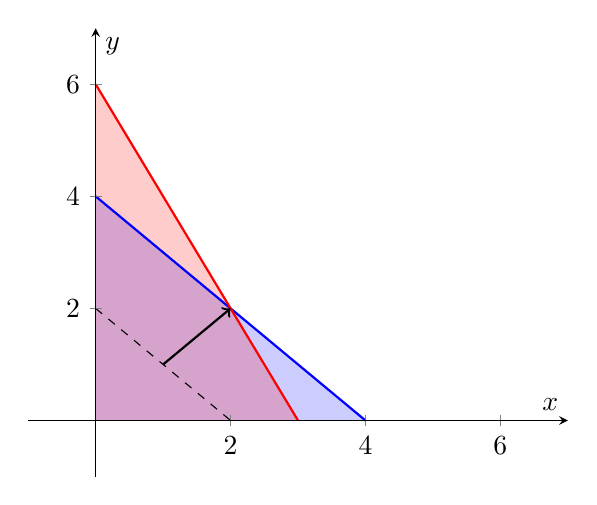
\begin{tikzpicture}
        \begin{axis}[
                xmin=-1, xmax=7,
                ymin=-1, ymax=7,
                axis lines=center,
                axis on top=true,
                domain=0:7,
                ylabel=$y$,
                xlabel=$x$,
                legend pos=north east, % Position for the legend
                legend cell align=left
            ]

            % Feasible regions with semi-transparent colors
            \addplot[fill=blue, fill opacity=0.2, draw=none, domain=0:4] {4-x} \closedcycle;
            \addplot[fill=red, fill opacity=0.2, draw=none, domain=0:3] {6-2*x} \closedcycle;



            % Inequalities
            \addplot[thick, domain=0:4, blue] {4-x};
            \addplot[thick, domain=0:3, red] {6-2*x};

            % Objective function (z = 3x + 2y = 12 as an example)
            \addplot[dashed, domain=0:2, black] {2-x};
            \draw[->, thick, black] (axis cs:1,1) -- (axis cs:2,2);

            % Dummy plots for legend
            \addplot[thick, domain=0:4, blue, forget plot] coordinates {(0,0)};
            \addplot[thick, domain=0:3, red, forget plot] coordinates {(0,0)};
            \addplot[dashed, domain=0:2, black, forget plot] coordinates {(0,0)};

        \end{axis}
    \end{tikzpicture}
    \caption{Feasible region of the LP problem, the area (purple) delimited by the constraint lines, blue and red. The dashed black line represents the objective function.}
\end{figure}\label{fig:lp_geom}

The simplex algorithm that we will descibe later starts at an initial feasible vertex and moves along the edges of the polytope to vertices with better objective values until the optimal vertex is reached.

\subsection{Feasibility, unboundedness}\label{feasibility}
We described how in geometric terms, a LP problem is feasible if the polytope defining its feasible region $ \chi $ is not empty. In other words, the LP is infeasible if no feasible solution exists, or $\chi = \emptyset$.

The LP is said to have unbounded set of solutions if its solution can be made infinitely large without violating any of its constraints. Meaning its feasible region is infinite, or unbounded. An example is shown in Figure \ref{unbounded}.

\begin{figure}[h]
    \centering
    \begin{tikzpicture}
        \begin{axis}[
                xlabel=\(x_1\),
                ylabel=\(x_2\),
                xmin=-1, xmax=5,
                ymin=-1, ymax=5,
                grid=both,
                minor tick num=1,
                major grid style={gray!30},
                minor grid style={gray!10},
                axis lines=middle,
                enlargelimits={abs=0.5},
                legend pos=north west,
            ]

            % Constraints
            \addplot[name path=constraint1, blue, thick, domain=0:5] {x + 1}; % x1 - x2 >= 1
            \addplot[name path=axis, draw=none, domain=0:5] {0}; % x-axis
            \addplot[blue!20] fill between[of=constraint1 and axis, soft clip={domain=0:5}];

            % Objective function (for illustration, let's assume z=3)
            \addplot[green, thick, dashed, domain=0:4] {3-x}; % x1 + x2 = 3

            % Arrow for objective function
            \draw[->, thick, green] (2,1) -- (3,0); % Arrow for the objective function

            % \legend{
            %    \(x_1 - x_2 \geq 1\),
            %    Objective function
            %}

        \end{axis}
    \end{tikzpicture}
    \caption{Graphical representation of an unbounded LP problem}
    \label{unbounded}
\end{figure}

The LP has an optimal solution, if there is a vertex \( \mathbf{x^*} \), called the optimal
vertex, such that
$\mathbf{c}^T \mathbf{x} \leq \mathbf{c}^T \mathbf{x^*} $ for all $\mathbf{x} \in \chi$.

\begin{figure}[!htb]
    \centering
    \begin{tikzpicture}[node distance=2cm, auto]
        % Define styles
        \tikzstyle{block} = [rectangle, draw, fill=blue!20, text width=6em, text centered, rounded corners, minimum height=3em]
        \tikzstyle{line} = [draw, -latex']

        % Place nodes
        \node [block] (basis) {Optimal Basis};
        \node [block, right=of basis] (solution) {Optimal Solution};
        \node [block, right=of solution] (vertex) {Optimal Vertex};

        % Draw edges
        \path [line] (basis) -- node {defines} (solution);
        \path [line] (solution) -- node {is} (vertex);

    \end{tikzpicture}
    \caption{Conceptual relationship between an optimal basis, an optimal solution,
        and an optimal vertex.}
\end{figure} \label{equivalence_terms}

\subsection{The Standard Simplex Algorithm}

In this subsection we will present the most widely used algorithm for solving LP problems, the simplex algorithm, as introduced by George Dantzig in 1947 \parencite{dantzig1990origins}.

\subsubsection{Computational form of LP}

To be approachable by the simplex algorithm, the LP problem \ref{LP_Problem} needs to be cast in a computational or standard form \ref{LP_Problem_Comp}, that fulfills the requirement of the constraint matrix having to have full row rank and only equality constraints are allowed. To convert the inequalities to equations, we introduce slack variables \(s_1, s_2, \dots, s_m\). After introducing those variables, we look at the problem \ref{LP_Problem}, where the constraints are now linear equalities:

\begin{align}
    \text{Maximize} \quad   & z = \mathbf{c}^T \mathbf{x} \notag                            \\
    \text{subject to} \quad & \sum_{j=1}^{n} a_{1j} x_j + s_1 = b_1 \notag                  \\
                            & \sum_{j=1}^{n} a_{2j} x_j + s_2 = b_2 \notag                  \\
                            & \vdots \notag                                                 \\
                            & \sum_{j=1}^{n} a_{mj} x_j + s_m = b_m \label{LP_Problem_Comp} \\
                            & x_1, x_2, \dots, x_n, s_1, s_2, \dots, s_m \geq 0 \notag
\end{align}

We then have a LP problem in the appropriate form and can be used as input for the simplex algorithm. To develop an intuition for how this algorithm works, it is helpful to view the strategy of the simplex algorithm as that of successive improvements until reaching an optimum \parencite{chvatal1983linear}. For instance, a maximization problem is optimized when the slack variables are “squeezed out,” maximizing the true variables’ effect on the objective function.

\subsubsection{Defining a Basis}
So far we have used the terms optimal vertex and solution interchangeably to refer
to the point that delivers the optimum of a LP problem, if plugged in the objective function. Now we will explore the concept of feasible and optimal basis. All the concepts are however equivalent, see \ref{equivalence_terms}. Yet the simplex algorithm uses the basis terminology.

In linear algebra, a basis of a vector space is a set of vectors that:
\begin{itemize}
    \item Spans the space: this means that every vector in the vector space
          can be expressed as a linear combination of the basis vectors.
    \item Is linearly independent: this means that no vector in the basis can be
          expressed as a linear combination of the other basis vectors.
\end{itemize}

If an LP problem has an optimal solution, then it is enough to search the finite number of vertices of the feasible region. Every vertex, or corner point of the feasible region has at least one set of $m$ linearly independent columns of $A$ associated with it. The set of indices of these columns is called a basis.

A basis can be seen as a basis matrix, consisting of the $m$ linearly independent columns of $\mathbf{A}$ associated with it.

Basic variables are the indices contained in a basis. A feasible basis is a basis for which all the basic variables have non-negative values when the other variables (non-basic variables) are set to zero in the constraints.

\subsubsection{The algorithm}
As we have seen, slack variables are introduced to convert inequalities into equations, and these slack variables can form an initial feasible basis. In this case, the decision variables are set to zero, and the slack variables are set to the values on the right-hand side of the constraints. This provides a starting point for the simplex method.

If the the right-hand side is a vector of nonnegative numbers, i.e. $\mathbf{b} \geq 0 $, then
the problem is said to be initially feasible.


\begin{algorithm}
    \caption{Simplex Algorithm}
    \begin{algorithmic}[1]
        \Procedure{Simplex}{$\mathbf{c}, \mathbf{A}, \mathbf{b}$}
        \State Initialize a feasible basic solution
        \While{true}
        \State Search for an entering variable (pricing)
        \If{no entering variable exists}
        \State \Return "Optimal solution found"
        \EndIf
        \State Search for a leaving variable using the minimum ratio test
        \If{no positive pivot element in the column}
        \State \Return "Unbounded"
        \EndIf
        \State Perform the pivot operation
        \State Update the basic and non-basic variables
        \EndWhile
        \EndProcedure
    \end{algorithmic}
    \label{algo:simplex_tableau}
\end{algorithm}


Let's present the methods used to perform the exchange in each step, i.e. the choice of the entering
variable and the choice of the leaving variable.

\begin{itemize}
    \item Pricing: The choice of the entering variable: we choose a non-basic variable to enter the basis
          and thus become basic. This is called Pricing. The choice usually depends on metrics
          like the largest increase in the objective function, or the largest coefficient.
          Bland's rule has been proved to guarantee termination and it states as follows:
          Choose the entering variable as the non-basic variable with
          the smallest index that has a negative reduced cost for a maximization problem:
          \[
              j = \min \{ j : c_j < 0 \}
          \]
          If there are no candidates for entering variable, we have reached the optimum.
    \item Ratio test: the choice of the leaving variable: we choose a basic variable to leave the basis:
          we do this by performing a ratio test.
          For the chosen entering variable, compute the ratios for all positive values in its column:
          \[
              \text{ratio}_i = \frac{b_i}{a_{ij}}
          \]
          Choose the leaving variable as the basic variable  has the smallest non-negative ratio.
          If there are no positive values in entering column, the problem is unbounded.
\end{itemize}

After selecting an entering variable and a leaving variable, we perform pivoting, or
updating the tableau. This is done through row operations \parencite{chvatal1983linear}.

\subsubsection{Termination}
\begin{enumerate}
    \item \textit{Optimality:}
          The algorithm terminates when there are no more negative coefficients in the objective function
          row for a maximization problem (or no more candidates for entering variables).

    \item \textit{Unboundedness:}
          If all the entries in the column of the entering variable are non-positive during the pivot
          operations, the problem is unbounded.

    \item \textit{Cycling:}
          The algorithm might enter a cycle, revisiting the same basic feasible solutions. Bland's rule
          can prevent this.

    \item \textit{Maximum Iterations:}
          A set maximum number of iterations can be used to prevent indefinite running due to
          numerical issues or other unforeseen circumstances. We set a bound on number of steps in our
          implementations. This bound is equal to the maximum value a 32-bit unsigned integer can take, or
          $4294967295$.
\end{enumerate}

\subsubsection{The runtime complexity of the simplex algorithm}
%Worst case vs. average case
Since the idea of the simplex algorithm is to search the finite number of bases until a basis is
found that belongs to the optimal vertex, and there are $\binom{m}{n}$ bases, this might take an exponential number of steps. In fact, Klee and Minty (1972) \parencite{klee1972good} constructed a worst-case example where $2^m -1$ iterations may be required, making the simplex' worst-case time complexity exponential, which we denote by \( O(2^m) \).

It can be however argued that this is only one worst-case example. Indeed, the number
of iterations usually encountred in practice or even in formal experimental studies of is much lower.
With $m<50$ and $m+n<200$, where $m$ and $n$ are the number of constraints and variables in the LP problem respectively, Dantzig \parencite{dantzig1990origins} observed that the number of iterations is usually less than $3m/2$
and only rarely going to $3m$. However, there is no proof that for every problem the simplex algorithm for linear programming has a number of iterations or pivots that is majorized by a polynomial function.

For packing linear programs, the worst-case time complexity of the simplex algorithm remains exponential, though there exist polynomial implementations in practice \parencite{stille2010solution}.

\subsubsection{Time complexity analysis of one step}
Given a linear program with \( m \) constraints and \( n \) variables, the tableau for the
simplex algorithm will be of size \( (m+1) \times (n+m+1) \).
The time complexity of one iteration of the tableau simplex algorithm can be broken down as follows:

\begin{itemize}
    \item Identifying the entering variable (choosing from $m$ non-basic variables): \( O(m) \)
    \item Identifying the leaving variable: \( O(n) \)
    \item Pivoting operation: \( O(m \times n) \)
\end{itemize}

Thus, the overall time complexity of one iteration is \( O(m \times n) \). This is considered large, especially knowing that there may be an exponential number of iterations. This is why we proceed to define other solution methods that succeeded to achieve a better time performance.

\subsection{The Interior Point Method}
The interior point method is another mathematical technique used to solve LP problems. Practically, this method is based on the idea of iteratively moving through the interior of the feasible region of the LP problem \parencite{alizadeh1995interior}. Mathematically, it can be described as follows:

Consider an LP problem in standard form:

\[
    \begin{aligned}
        \text{minimize:} \quad   z = & \mathbf{c}^T\mathbf{x}   \\
        \text{Subject to:} \quad     & \mathbf{Ax} = \mathbf{b} \\
                                     & \mathbf{x} \geq 0
    \end{aligned}
\]

The interior point method introduces a penalty function to the objective function, which discourages solutions near the boundary of the feasible region. This barrier function is typically defined as $-\sum \log(x_i)$, where $x_i$ represents the elements of the vector $x$.
The optimization problem then becomes:

\[
    \begin{aligned}
        \text{Minimize:} \quad & c^Tx - \mu \sum \log(x_i)
    \end{aligned}
\]

The key mathematical insight of the interior point method is that as $\mu$ approaches zero, the solution converges toward the optimal solution of the original LP problem. The method iteratively updates $\mu$ and the solution vector $\mathbf{x}$ until a suitable solution within the interior
of the feasible region is found.

\subsubsection{Time Complexity Analysis}
The time complexity of the interior point method for linear programming is determined by the number of iterations required for convergence. In practice, the number of iterations is often polynomial in
the problem size, which includes the number of decision variables $n$ and constraints $m$.
Each iteration involves solving a system of linear equations, for example: $Hd = -(c + A^T\lambda)$. A mathematical derivation of this equation can be found in literature \parencite{alizadeh1995interior}.

Where:
\begin{itemize}
    \item $H$ is a symmetric positive definite matrix.
    \item $d$ is the Newton direction.
    \item $c$ is the vector of coefficients representing the objective function.
    \item $A$ is the constraint matrix.
    \item $\lambda$ is the vector of dual variables.
\end{itemize}


Solving this system can be done efficiently, especially if $H$ and $A$ are sparse (e.g. using Cholesky, LU decomposition \parencite{golub2013matrix}).
We can express the overall time complexity of the interior point method as follows:

\[
    O(k \cdot (f(n, m) + g(n)))
\]

Where:
\begin{itemize}
    \item $m$ and $n$ represent the size of the LP
    \item $k$ is the number of iterations.
    \item $f(n, m)$ represents the cost per iteration, which is polynomial in $n$ and $m$.
    \item $g(n)$ represents any additional preprocessing or initialization costs, which are typically polynomial in $n$.
\end{itemize}
Therefore, the overall time complexity of the interior point method is polynomial $n$ and $m$, number of variables and constraints in the LP, respectively. This is better than the (worst-case) exponential time complexity of the simplex algorithm.

\subsection{Revised Simplex Algorithm}
While the standard or tableau simplex algorithm maintains and updates theentire tableau in its
dense form at each iteration, and the pivotting step of this algorithm is highly costly as we have to update the entire matrix using row operations. The revised simplex method transforms only the inverse of the basis matrix, $mathbb{B}^{-1}$, thus reducing the amount of writing at each step and overall memory usage.

\subsubsection{The algorithm}
Let's derive the mathematical proof of this algorithm:
Given a linear programming problem in standard form:
\begin{align*}
    \text{maximize} \quad   & \mathbf{c}^T \mathbf{x}           \\
    \text{subject to} \quad & \mathbf{A}\mathbf{x} = \mathbf{b} \\
                            & \mathbf{x} \geq \mathbf{0}
\end{align*}
where \(\mathbf{A} \) is an \( m \times n \) matrix,
\( \mathbf{b} \) is an \( m \times 1 \) vector, and
\( \mathbf{c} \) is an \( n \times 1 \) vector.


Partition \( \mathbf{x} \) into basic (\(\mathbf{x}_B \)) and non-basic (\( \mathbf{x}_N \)) variables.
As mentioned before, basic variables are the indices contained in a basis. A feasible basis is a basis for which
all the basic variables have non-negative values when the other variables (non-basic
variables) are set to zero in the constraints.
Similarly, partition \( \mathbf{A} \) into \( \mathbf{B} \) (columns corresponding to \( \mathbf{x}_B \))
and \( \mathbf{N} \) (columns corresponding to \( \mathbf{x}_N \)).

The constraints can be written as:
\begin{align*}
    \mathbf{B}\mathbf{x}_B + \mathbf{N}\mathbf{x}_N & = \mathbf{b} \\
    \mathbf{x}_B                                    & \geq 0       \\
    \mathbf{x}_N                                    & \geq 0
\end{align*}

From \( \mathbf{B}\mathbf{x}_B + \mathbf{N}\mathbf{x}_N = \mathbf{b} \), when \( \mathbf{x}_N = 0 \):
\[ \mathbf{x}_B = \mathbf{B}^{-1}\mathbf{b} \]
This is the basic feasible solution if all entries of \( \mathbf{x}_B \) are non-negative.

Compute the reduced costs:
\[ \bar{\mathbf{c}}_N^T = \mathbf{c}_N^T - \mathbf{c}_B^T \mathbf{B}^{-1} \mathbf{N} \]
If all entries of \( \bar{\mathbf{c}}_N^T \) are non-negative,
then the current basic feasible solution is optimal.

If some entries of \( \bar{\mathbf{c}}_N^T \) are negative,
choose \( j \) such that \( \bar{c}_j < 0 \). Compute:
\[ \mathbf{d} = \mathbf{B}^{-1} \mathbf{A}_j \]
If all entries of \( \mathbf{d} \) are non-positive, the problem is unbounded.

Otherwise, compute the step length:
\[ \theta = \min \left\{ \frac{\mathbf{x}_B[i]}{\mathbf{d}[i]} : \mathbf{d}[i] > 0 \right\} \]
Update the solution:
\[ \mathbf{x}_B = \mathbf{x}_B - \theta \mathbf{d} \]
\[ x_j = \theta \]
and update the sets of basic and non-basic variables.

This proof elucidates that the only variables required to "recreate" exactly the tableau at
each step, without performing the costly pivotting operation are:
\begin{itemize}
    \item the indices of basic and non-basic variables.
    \item $B^{-1}$ the inverse of the basis matrix. This is used to solve two types of linear equations
          during an iteration, see step 1 and 3 in Algortihm \ref{algo:revised}.
          In the actual implementation, there is no need to compute or store the $B^{-1}$.
          We just use the basis matrix $B^{-1}$ to solve these linear systems of
          equations. Therefore in practice, we only store $B$.
    \item the current values of the basic variables, or the current basic feasible solution. $x_B = B^{-1}b$
\end{itemize}

The algorithm is elaborated in \ref{algo:revised}. As we can see, step 1 and 3 represent the solving of two types of systems, Forward Transofrmation (FTRAN) and Backward Transofrmation (BTRAN).

However, having to recompute the inverse of a matrix, or in our actual
implementation, solve a linear equation system may be costly.

\subsubsection{Inverting a square matrix}
For a square matrix of size \(n \times n\), the time complexity of LU
decomposition
\parencite{golub2013matrix},
which is one of the
most prominent methods to invert a matrix, is $O(n^3) $.

This is why it is desirable to employ another tool to efficiently
update the inverse of the basis matrix $\mathbf{B}^{-1}$
without having to recompute it from scratch each time.
Such tools are called update methods,
and we will later describe the Product Form of the Inverse (PFI),
the Middle Product Form of the Inverse (MPFI) and we also describe Forrest-Tomlin update method
in the future work section.

\begin{algorithm}
    \caption{Revised Simplex Algorithm \parencite{chvatal1983linear}}
    \begin{enumerate}
        \item \textbf{Input:} A feasible basic solution, \( \mathbf{B} \), \( \mathbf{c} \), \( \mathbf{A} \), and \( \mathbf{b} \)
        \item \textbf{Output:} Optimal solution or a certificate of unboundedness
        \item Initialize \( \mathbf{B}^{-1} \), the inverse of the basis matrix \( \mathbf{B} \)
        \item \textbf{While True:}
              \begin{itemize}
                  \setlength{\itemindent}{3em}
                  \item[\textit{Step 1:}] Solve the system \( y\mathbf{B} = \mathbf{c}_B \) (BTRAN)
                  \item[\textit{Step 2:}] Choose an entering column. This may be any column $\mathbf{a}$  of
                      \( \mathbf{A}_N \) such that \( y\mathbf{a} \) is less than the corresponding component
                      of \( \mathbf{c}_N \). If there is no such column, then the current solution is optimal, Break.
                  \item[\textit{Step 3:}] Solve the system \( \mathbf{B}\mathbf{d} = \mathbf{a} \) (FTRAN)
                  \item[\textit{Step 4:}] Let \( \mathbf{x}_B^{\ast} = \mathbf{B}^{-1}\mathbf{b} \) the current basic variables' values.
                      Find the largest \( t \) such that \( \mathbf{x}_B^{\ast} - t\mathbf{d} \geq 0\)
                      if there is no such \( t \), then the problem is unbounded, Break; otherwise, at least
                      one component of  \( \mathbf{x}_B^{\ast} - t\mathbf{d} \) equals zero and the corresponding variable is leaving the basis.
                  \item[\textit{Step 5:}] Set the value of the entering variable at
                      \( t \) and replace the values \( \mathbf{x}_B^{\ast} \) of the basic variables by \( \mathbf{x}_B^{\ast} - t\mathbf{d} \).
                      Replace the leaving column of \( \mathbf{B} \) by the entering column, and in the basis heading,
                      replace the leaving variable by the entering variable.
              \end{itemize}

        \item \textbf{Return} Optimal solution \( \mathbf{B}^{-1}\mathbf{b} \)
    \end{enumerate}
    \label{algo:revised}
\end{algorithm}


\subsubsection{The product form inverse update method}

We will discuss the Product Form of the Inverse (PFI), introduced by
George Dantzig \parencite{dantzig1954product}. In the revised simplex method,
there is a need to represent the inverse of the basis matrix and efficiently
solve the BTRAN and FTRAN systems in Step 1 and 3 of Algorithm \ref{algo:revised}
in each iteration to find the entering and leaving variables.

To avoid the costly reinversion of the basis matrix in each step,
we apply an INVERT operation only once at the beginning, on the initial basis
matrix \(\mathbf{B}_0\). Inverting a matrix using LU decomposition requires \(O(n^3)\)
operations.

If \(\mathbf{B}_k\) denotes the basis matrix after \(k\)
iterations of the simplex method, and each \(\mathbf{B}_k\) differs from the
preceding \(\mathbf{B}_{k-1}\) in only one column, with index $p$, the entering index,
we have the following update equation:

\[
    \mathbf{B}_k = \mathbf{B}_{k-1}\mathbf{E}_k \label{eq:basis_update}
\]

with \(\mathbf{E}_k\) representing the identity matrix whose \(p\)th column
is replaced by \(\mathbf{d}\), and is referred to as an \textit{eta matrix}.
Consequently, when the initial basis consists of slack variables,
we have \(\mathbf{B}_0 = \mathbf{I}\), and successive applications of
Equation \ref{eq:basis_update} yield:

\[
    \mathbf{B}_k = \mathbf{E}_1\mathbf{E}_2 \cdot \mathbf{E}_k \label{eq:eta_factorization}
\]

This eta factorization of \(\mathbf{B}\) provides an optimized way
to solve the two systems.

Solving the system \(y\mathbf{B}_k = \mathbf{c}_B\) comes down to solving:

\[
    (((y\mathbf{E}_1)\mathbf{E}_2) \ldots )\mathbf{E}_{k} = \mathbf{c}_B
\]

Solving the system \(\mathbf{B}_kd = \mathbf{a}\) comes down to solving:

\[
    \mathbf{E}_1(\mathbf{E}_2( \ldots (\mathbf{E}_{k}\mathbf{d}))) = \mathbf{a}
\]

\textbf{Time complexity of direct solution:}
Solving the system \(y\mathbf{B}_k = \mathbf{c}_B\) or \(\mathbf{B}_k\mathbf{d} = \mathbf{a}\) directly using
Gaussian elimination or LU decomposition has a time complexity of \(O(m^3)\),
where \(m\) is the dimension of \(\mathbf{B}_k\), i.e. the number of constraints in the LP.

\textbf{Time complexity using eta factorization:}
Solving \(\mathbf{C}_i x = y\) or  \(\mathbf{x}\mathbf{E}_i = y\) involves
simple vector operations and matrix multiplication,
which has a time complexity of \(O(n^2)\).
Therefore, applying \( \mathbf{B}_k = \mathbf{E}_1 \mathbf{E}_2 \ldots \mathbf{E}_k\)
takes a time complexity of \(O(kn^2)\), where $k$ is the number of eta vectors,
or the current iteration count.

\textbf{Comparing the Two Methods:}
\begin{itemize}
    \item Direct Solution: \(O(m^3)\) for both systems.
    \item Using Eta Factorization: \(O(km^2)\) for both systems,
          where \(k\) is the number of iterations.
\end{itemize}

In summary, when using the eta factorization method,
the time complexity for solving both systems becomes \(O(km^2)\),
which depends on the number of iterations (\(k\)) and the number of
constraints (\(m\)).

\subsubsection{The modified product form inverse}
The Middle Product Form (MPF) update is a variant of the PFI that integrates
updates in product form into the middle of factors L and U.
This update
is described mathematically in literature \parencite{huangfu2015novel}. This variant
has also been proved empiricially to have a better performance than PFI and other PFI variants.
This is also the update method used in Umbra's cardinality estimator \parencite{Umbra}.

\section{Cardinality Estimation}\label{section:cardinality-estimate}
An important use case of linear programming solvers in the field of database systems is
cardinality estimation.
In the context of query optimization, LP solvers can be useful to estimate query plan
cardinalities and provide a reliable and good enough estimate to be used in selecting
the best join order, and hence speeding up query execution time \parencite{leis2018query}.

Cardinality, defined as the number of tuples in the output,
plays a pivotal role in the selection of an optimal query plan.
Modern DBMS often rely on
cost-based query optimizers to make this selection.
For example, the SQL Server Query Optimizer
\parencite{microsoft2023cardinality} employs a
cost-based approach, aiming to minimize the estimated
processing cost of executing a query.

Enhanced cardinality estimation
can lead to more accurate cost models, which in turn results
in more efficient query execution plans.
Consequently, accurate and reliable cardinality estimates are
crucial in achieving faster query execution times.
The objective is to develop a LP
solver designed specifically for cardinality estimation.
This solver aims to maximize a cost function that represents
the upper bound of the output size, optimizing for both
time and memory complexity.
We assume the worst-case join sizes, and want to see how large our variable domains
can be given this worst-case scenario.

To set the stage for our implementation, we introduce the AGM bound.

\subsection{AGM bound}
The AGM bound \parencite{atserias2013size} proves
using entropy that \[ \min_w \left( \sum_{i=1}^{k} w_i \log |R_i| \right) \]
is a tight upper bound for join size, given query graph (how the
relations are connected, if there are any shared attributes)
and relation sizes. The AGM bound is tight; in other words, we can always find
a database instance linked to this join size upper bound.
The dual LP problem of the given minimzation problem, is
\[ \max \sum_{i} v_i \]
subject to:
\[ A^T \mathbf{v} \leq \log |R| \]
The dual theorem \ref{duality} states that the both problems have the same
optimal values.

This is how our query LP datasets are generated.
Umbra cardinality estimation utilizes pessimistic estimates, that guarantee that the cardinalities will not exceed that bound.

To elucidate the core concepts,
suppose we have two relation $R$ and $S$ with attributes
\[
    Q(a, b, c) = R(a, b) \Join S(b, c)
\]
where we denote the sizes of the relations as
$|R|$ and $|S|$ respectively.
It is easy to see that the largest possible output is $|R| \cdot |S|$, which occurs when the join
behaves like a cartesian product, i.e. have a selectivity equals to 1. So, this is the worst-case
upper bound.

Deriving a simple example for an LP problem related to cardinality estimation leads us to the inequality \ref{eq:initial_inequality}. Applying the natural logarithm to both sides yields \ref{eq:log_inequality}. We then rename the variables, simplifying the inequality to \ref{eq:renamed_inequality}.
Normalizing by dividing both sides by \(r'\), we obtain \ref{eq:normalized_inequality}. This leads us to the objective function for our packing LP problem.
\begin{align}
    |a| \cdot |b|                            & \leq |R| \label{eq:initial_inequality}                                                   \\
    \ln|a| + \ln|b|                          & \leq \ln|R| \label{eq:log_inequality}                                                    \\
    a' + b'                                  & \leq r' \label{eq:renamed_inequality}                                                    \\
    \frac{1}{r'} a' + \frac{1}{r'} b'        & \leq 1 \label{eq:normalized_inequality}                                                  \\
    \text{maximize } a' + b' + c' + d' \quad & \text{s.t.} \quad \frac{1}{r'} a' + \frac{1}{r'} b' \leq 1 \label{eq:objective_function}
\end{align}

And in this simple abstracted way we get a sample packing LP from our dataset, where the decision variables would be the logarithms of the domains sizes of our variables, Our objective if to maximize the sum of our variables, and the constraints are the ones imposed by the AGM bound.

\section{State-of-the-art LP solvers}
Here we will discuss alternative approaches that are used today to solve LPs. Nowadays, the best
existing open-source and commercial LP-systems are based on implementations that make use
of various algorithms and techniques to speed up the solution of large scale LP problems.
There exist various LP solvers today, like CPLEX (IBM), CBC, Gurobi, HiGHS... We present HiGHS Scipy, and
Cplex, because we are using them as a comparison to our solvers.
\subsection{HiGHS Scipy}
HiGHS, or High Performance Optimization Software is a software used to define,
modify and solve large scale sparse linear optimization models.

For LPs, HiGHS has implementations of both the revised simplex and interior point methods
\parencite{Huangfu2018}.
HiGHS has primal and
dual revised simplex solvers, originally written by Qi Huangfu and
further developed by Julian Hall.
In our comparison, we do not make use of HiGHS directly but through Scipy's linprog, and using the solver as a method. It is mainly used to verify the accuracy of the optimal values
obtained by our solvers.

\begin{lstlisting}[language=Python]
    linprog(method='highs')
\end{lstlisting}

\subsection{Cplex}
IBM ILOG CPLEX Optimization Studio, commonly known as CPLEX,
is a software suite for mathematical optimization \parencite{cplex2009v12}.
CPLEX consists of a library for linear programming,
mixed integer programming, quadratic programming, and other optimization problems.

CPLEX utilizes a variety of algorithms to tackle linear programming (LP) problems.
Although the majority of LP instances are efficiently solved using CPLEX's
cutting-edge dual simplex algorithm, there are cases where other algorithms might be more suitable.
For certain problem types, the primal simplex algorithm and the interior point method.

Furthermore, CPLEX provides a concurrent option, which runs multiple algorithms in parallel,
returning the solution from the first algorithm to complete.
It also supports various interfaces, including C++, Java, and Python. In our experiments
we use the python interface.
CPLEX is widely used in both academia and industry for solving large-scale optimization
problems.
